\documentclass{beamer}
\usepackage[utf8]{inputenc}
\usepackage[T1]{fontenc}
\usepackage[english]{babel}
\usepackage{amssymb}
\usepackage{soul}
\usepackage{listings}
\usepackage{alltt}
\usepackage{underscore}
\usepackage{verbatim}
\usepackage{graphicx}
\usepackage{ae}
\usepackage{amsmath}
\usepackage{amsfonts}
\PassOptionsToPackage{pdflatex}{graphicx}
\usepackage{algorithm}
\usepackage{algorithmic}
\graphicspath{ {images/} }

\definecolor{listinggray}{gray}{0.9}
\definecolor{lbcolor}{rgb}{0.9,0.9,0.9}


\usefonttheme{professionalfonts}


\title[Degree Project]{Degree Project}
\subtitle{Presentation \#1} 
\author[E. Regla]{Erik Regla} 
\institute[UTalca]{Universidad de Talca}
\date{\today} 

\begin{document}

\begin{frame}
  \titlepage
\end{frame}

\section{Descripción de las pruebas experimentales}

\begin{frame}
  \begin{itemize}
  	\item Advisor: Rodrigo Paredes (rapa)
  	\item Thema: Worst-Case optimal incremental sorting for discrete classes
  	\item Current Status: A paper. Initial tests and code ready. Pending documentation.
  	\item Motivation: Everyone loves to talk big about algorithms, but no one actually implements them.
  \end{itemize}
\end{frame}

\begin{frame}
    \centering
    \begin{figure}
        \includegraphics[height=.4\textheight]{IQS}\\
        \caption{IQS algorithm as published in 10.1007/s00453-010-9400-6}
    \end{figure}
\end{frame}

\begin{frame}
    \centering
    \begin{figure}
        \includegraphics[height=.6\textheight]{IIQS}\\
        \caption{IQS algorithm as published in 10.1109/SCCC.2015.7416566}
    \end{figure}
\end{frame}


\begin{frame}
    \centering
    \begin{figure}
        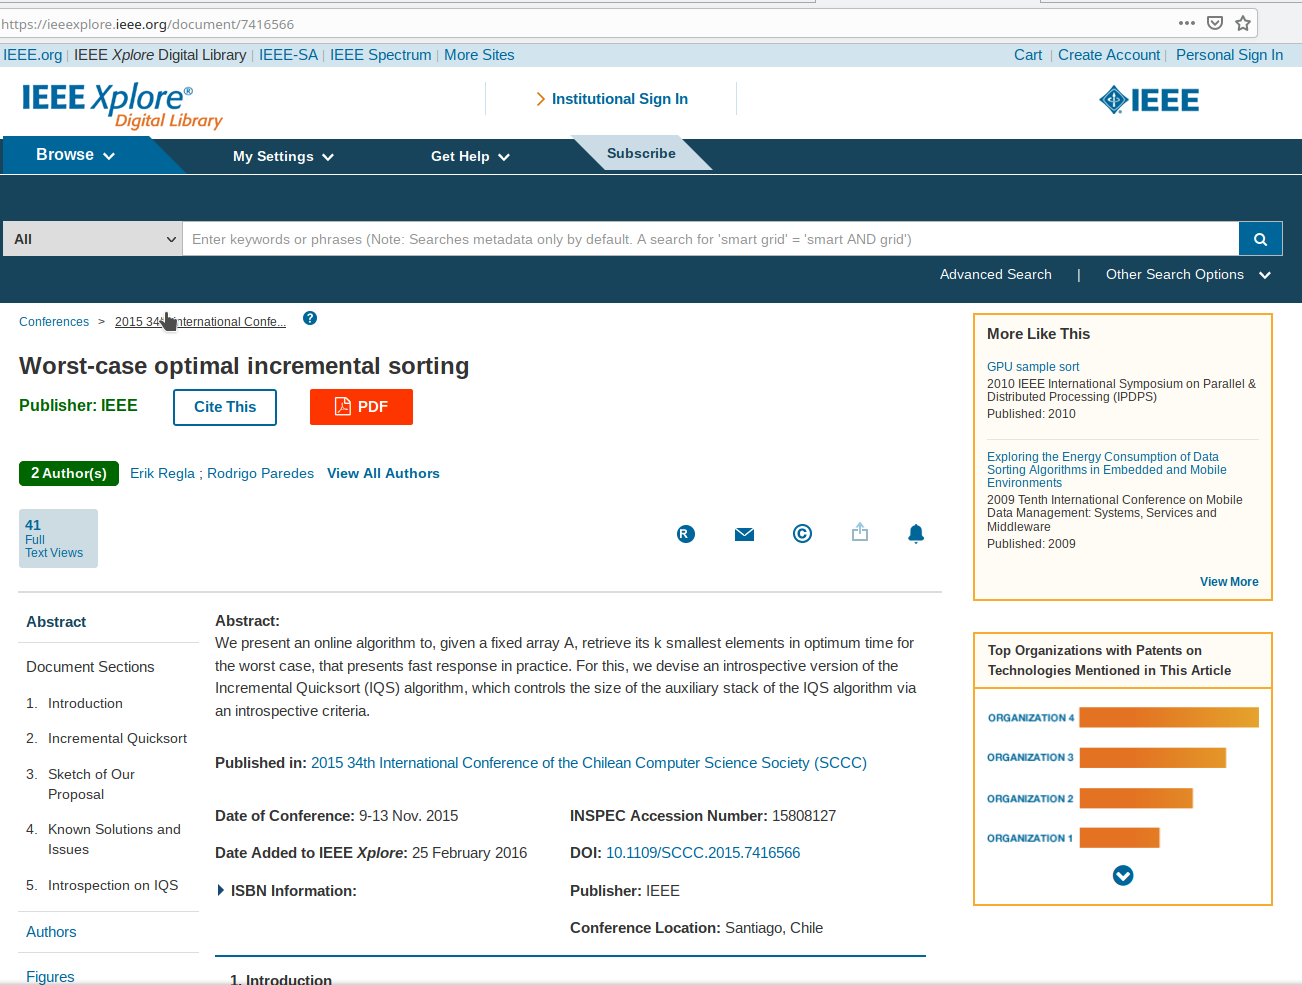
\includegraphics[height=.6\textheight]{paper}\\
        \caption{IIQS implmementation changes the partition method in order to guarantee a partition of linear time and at the same time guarantee a reduction on the search space. (10.1109/SCCC.2015.7416566).}
    \end{figure}
\end{frame}


\begin{frame}
    Current scope is limited as an experimental algorithm design \footnote{doi:10.1017/CBO9780511843747} to extend (I)IQS usage for haplotype plot\footnote{doi:10.1111/2041-210X.12747} generation, which is an instance of the worst case for IQS but on a discrete space when $C<<n$.
    \newline
    \newline

    Tested variants of the original implementation are as follows:
\begin{itemize}
    \item Test 1: Add incremental version of BFPRT algorithm% \pause Success
    \item Test 2: Change rules for introspective step% \pause Success
    \item Test 3: Bias the three-way-median returned index% \pause Success
    \item Test 4: Store the three-way-median result on the stack
    \item Test 5: Alter rules for storing pivots
\end{itemize}
\end{frame}

\begin{frame}
    The beforementioned changes can induce new problems and behaivours, known but not limited to stack size, cache trashing, non-existant DRAM bursting, memory corruption, etc.
\begin{itemize}
    \item Test 1: No changes to running speed, improved median selection with less memory ussage
    \item Test 2: Depends on the distribution (not applicable if it is not known).
    \item Test 3: Stabilization over running time and stack usage. Increased DRAM burst toll.
    \item Test 4: Cache and DRAM burst trashing on low-power devices. Trade-off between use cases as it doesn't perform on the general case.
    \item Test 5: Depends on the input distribution, useless if not combined with one of the former tests.
\end{itemize}
\end{frame}


\begin{frame}
    \centering
    \begin{figure}
        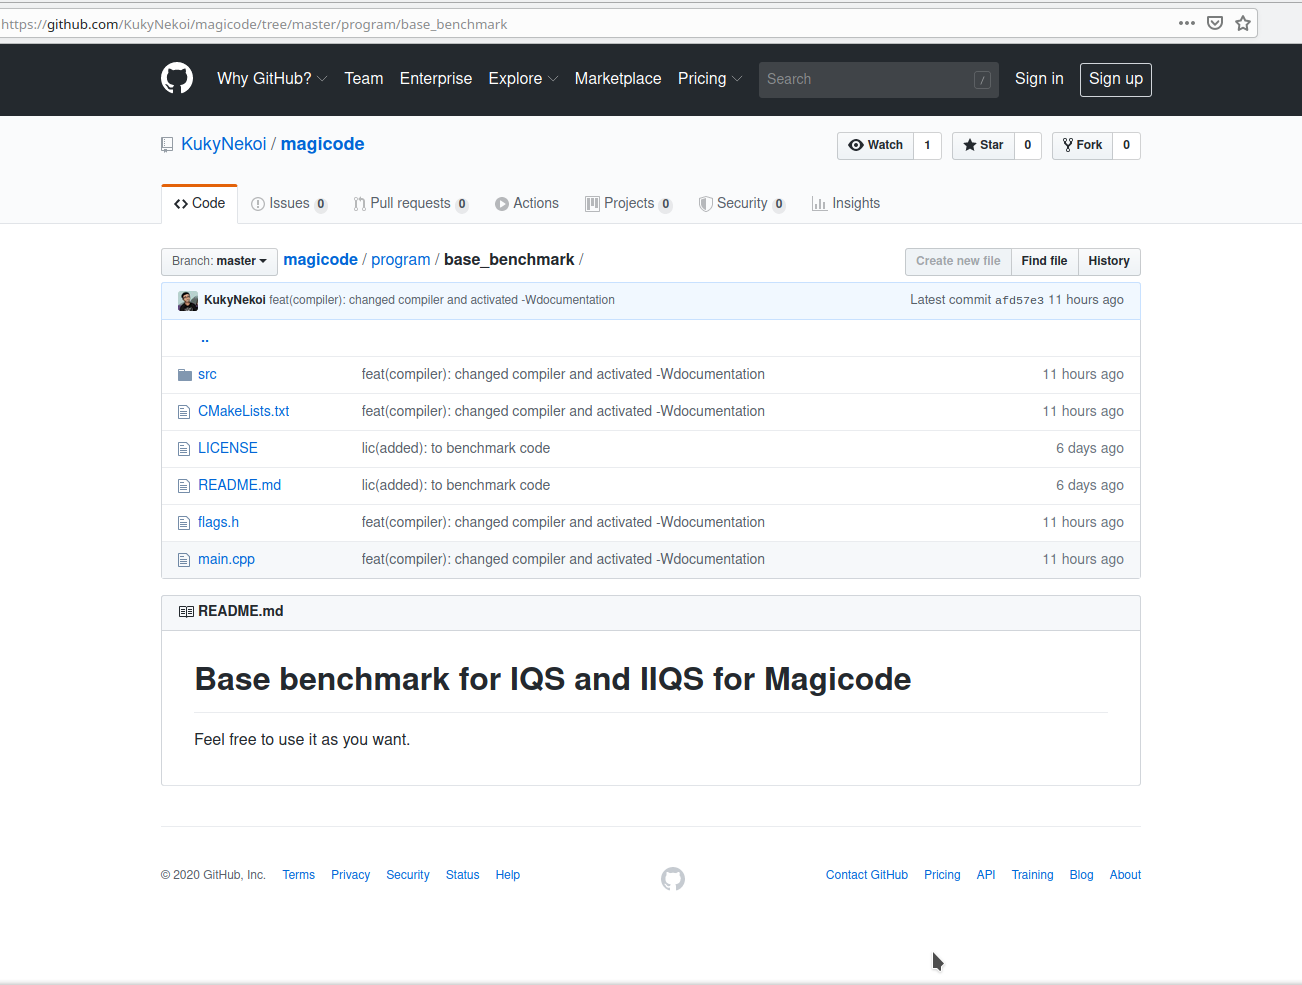
\includegraphics[height=.6\textheight]{repo}\\
        \caption{Implementation for the tests on C++ (STL-container-friendly implementations and without STL) available under GNU GPL license at \href{https://github.com/KukyNekoi/magicode/tree/master/program/base_benchmark}{GitHub}}
    \end{figure}
\end{frame}


\begin{frame}
\begin{itemize}
    \item Scope: Experimental design, setup and experimentation
    \item Part of magicode, a personal research on FPGA implementation of hardware accelerators for similarity search (the original thema).
    \item Got someone interested on using this algorithm for solving haplotype plots.
\end{itemize}
\end{frame}
  
\begin{frame}
\centering
		FIN
\end{frame}



\end{document}
